\documentclass[tikz]{standalone}
\usepackage{tikz}
\usepackage{fourier}
\usepackage{physics}
\usetikzlibrary{shapes.geometric}
\usetikzlibrary{calc}

\begin{document}
\begin{tikzpicture}
    \node[inner sep=0] at (0, 0) {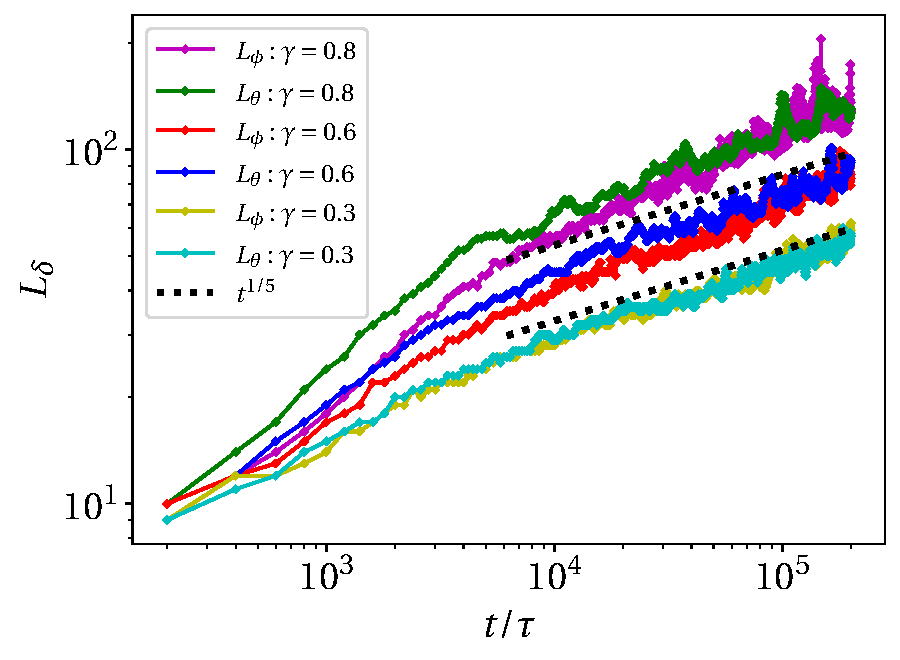
\includegraphics[scale=0.605]{gfx/correlation_lengths.pdf}};
    \node[inner sep=0] at (9.5, 0.05) {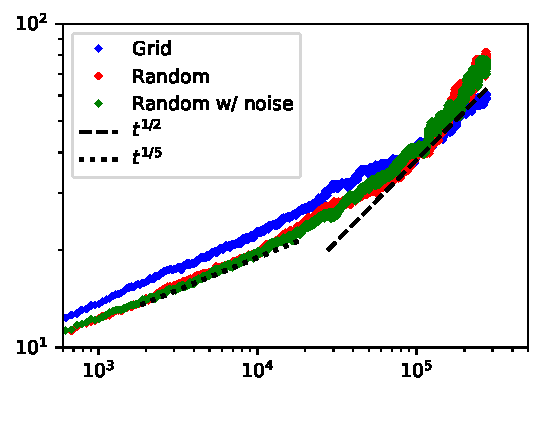
\includegraphics{gfx/scalar_vortex.pdf}};

    % Scalar labels
    \node at (10, -3) {\large \(t/\tau\)};
    \node[rotate=90] at (5.2, 0.55) {\large \(\ell_d\)};

    % Plot labels
    \node at (0.6, -3.7) {\large (a)};
    \node at (10, -3.7) {\large (b)};
\end{tikzpicture}
\end{document}
